\documentclass{article}

\usepackage[english]{babel}


\usepackage[a4paper,top=2cm,bottom=2cm,left=3cm,right=3cm,marginparwidth=1.75cm]{geometry}

\usepackage{amsmath}
\usepackage{graphicx}
\usepackage[colorlinks=true, allcolors=blue]{hyperref}

\title{Public history on social media}
\author{Toma-Stefan Cezar, Mourice Guscher, Joshua L. Lembke, Elias Gauger}

\begin{document}
\maketitle

\begin{abstract}
This article was not written under any scientific standard and is under no circumstances intended for use in any kind of further study due to a small sample size, limited time and lack of skills. Therefore the data could be biased. Using surveys and questions, which are further explained in following sections, we tried to show the amount of historical content on social media, using the platforms Instagram and TikTok. We found that historical content is present on social media and is being represented in a large variety of forms. The formats, which are used to convey historical, political or religious content, suggest that social media is a relevant field in "Public History".
\end{abstract}

\section{Introduction}
% add study "social media as Tools for Political Views Expressed in the Visuals Shared among social media Users"

Social media influences every ones life through sophisticated and complicated mechanisms, thus it has a major impact on historical, religious and maybe even political views. As already addressed in the Abstract we couldn't get a large amount of unbiased data, due to an limited amount of time, so this article should be interpreted not as an scientific paper, but rather as an article that aims to be an first effort at creating awareness about the topic. This whole article was written with the motivation of finding a direct connection between historical content on social media and the broad field of "Public History". Public History has infamously many definitions, therefore we will define our interpretation of "Public History". Public History is, for the scope of this article, history that is happening and being discussed outside of an specialized academic setting. According to this definition, social media seems like the ideal medium for Public History as it offers almost everyone an voice and has enormous popularity, especially among the younger generations.

\subsection{Objective}
 Our goal is it to show the amount of political and historical content presented to the average social media user between the ages of 13 and 21 years. Furthermore we tried to find the difference between the two social media platforms "TikTok" and "Instagram", especially regarding the format in which historical, political or religious content gets presented to the user. According to our surveys our participants have a mean average age of $\mu \approx 16.086$, this is important as it may indicate a bias.
 
%In what form does the political, historical or religious content appear

\begin{center}

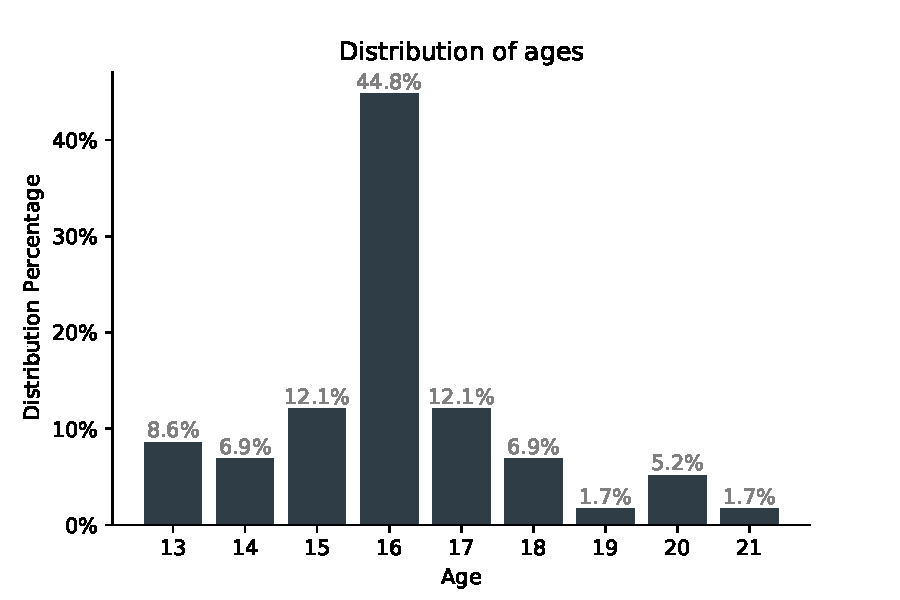
\includegraphics[scale = 0.75]{AgeGraph.pdf}

\end{center}

\subsection{Selection of social media platforms and age group}
Throughout this article we used the social media platforms "TikTok" and "Instagram" as reference, due to a large popularity and major coverage of the selected age group. The second reason for choosing said platforms and the earlier mentioned age group of 13-21 is the exclusion of academic groups, as this study is focusing on public history. According to the conducted survey, people are more likely to use TikTok more regularly compared to Instagram, yet Instagram has a higher overall usage compared to TikTok. 

\begin{center}

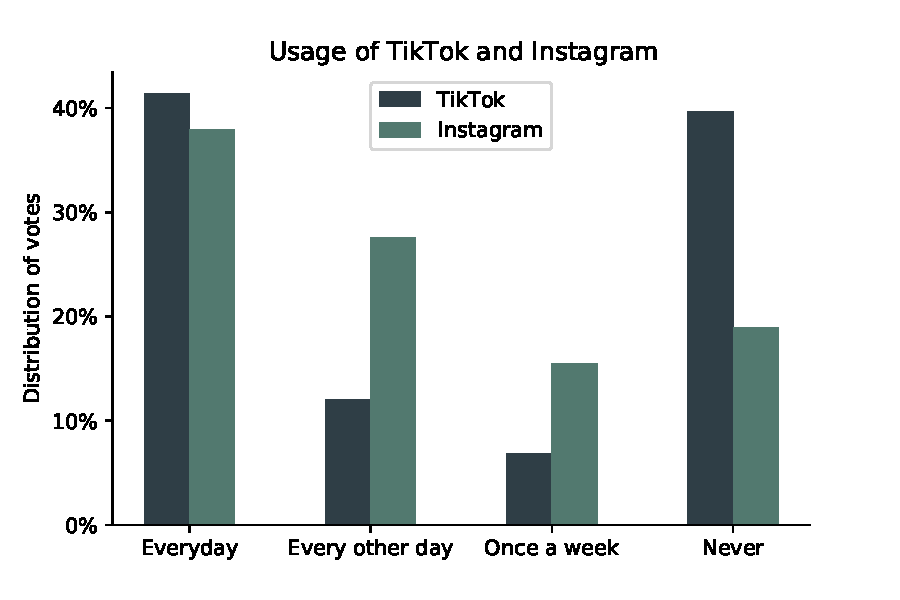
\includegraphics[scale = 0.65]{Usage.pdf}

\end{center}



\section{Methods}

Out data was gathered by a small research team in the form of anonymous surveys. There were two types of surveys, the first one was made using Google Forms and was sent to as many people as possible, the second one was an "Oral survey", that was conducted by the mentioned research team. Both surveys were translated from the original language (German) into English, in order to reach a broader field of people. The data got interpreted and visualised by one "hobby" computer scientist and was reviewed by the research team. The exact process of the interpretation and visualisation is explained in further detail on the Jupyter notebook. All of the data was visualised using Matplotlib and Google Colab. We surveyed a total of 58 people.

\subsection{Conclusion}

We found out that history, political and religious content is represented on both  
examined social media platforms. The following graph further shows the amount content existing on both platforms, this also shows that Public History is represented on social media. Important for the connection between social media and Public History is the fact that TikTok has, on average, more historical, political and religious content than Instagram. 

\begin{center}

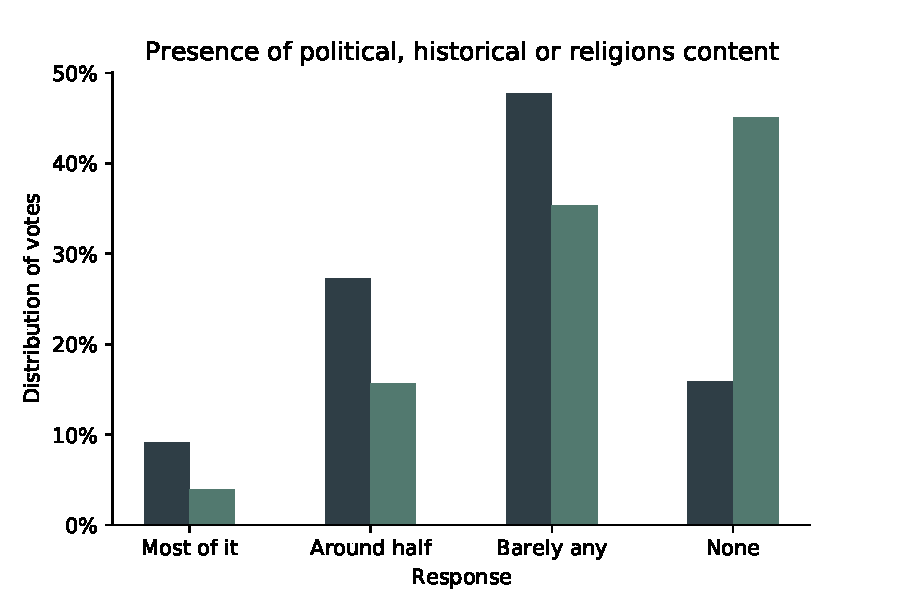
\includegraphics[scale = 0.65]{PresenceOfPHR.pdf}

\end{center}

We also analyzed the forms in which the content appears on social media. TikTok and Instagram again show a major difference. TikTok mostly represents historical, political and religious content in the form of "Entertaining Videos", "Informative Videos" and "Memes". Instagram on the other side represents the content in the form of  "Informative Videos", "Memes" and "Other". This again shows that Public History is mostly represented on social media. As "Memes" and "Entertaining Videos" are usually outside of an academic setting and should therefore be considered Public History.


\begin{center}

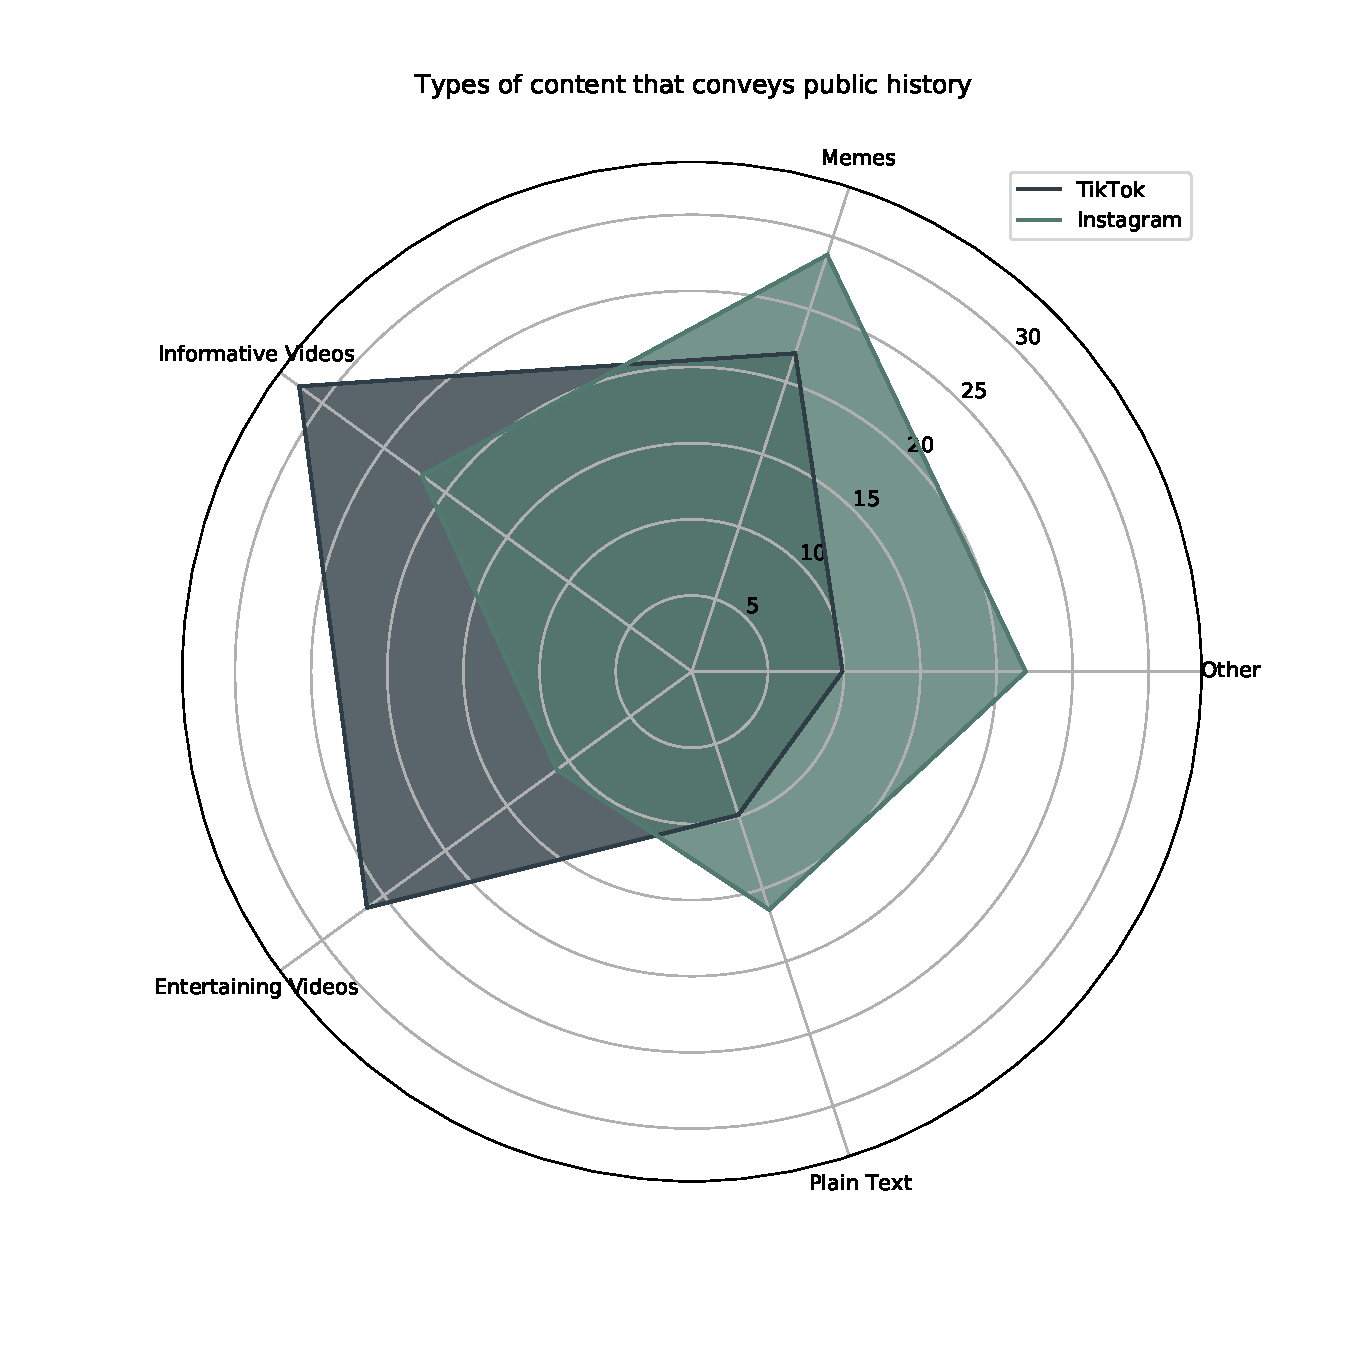
\includegraphics[scale = 0.6]{TypesOfContnent.pdf}

\end{center}

\newpage

\section{Links}
 

\url{https://github.com/StevenIGuess/Public-history-on-social-media/blob/main/Historical_content_on_Social_Media.ipynb}\\

\url{https://colab.research.google.com/drive/1YLO4dN-_yBXNIry-C64I_vWBYW9xEP2X?hl=de#scrollTo=XsS2n62k9xz0}\\

Surveys: \\

I \url{https://forms.gle/q7FZveMTPhYXcMUr6}\\

II \url{https://forms.gle/zJYcG8rpLFwPYe4K9}\\





\end{document}